\subsection{23 августа.  Пер. Джалпаккол Северный (1А)}
\textit{Метеоусловия: утром: ясно, тепло, потом??????????}

\begin{figure}[h!]
	\centering
	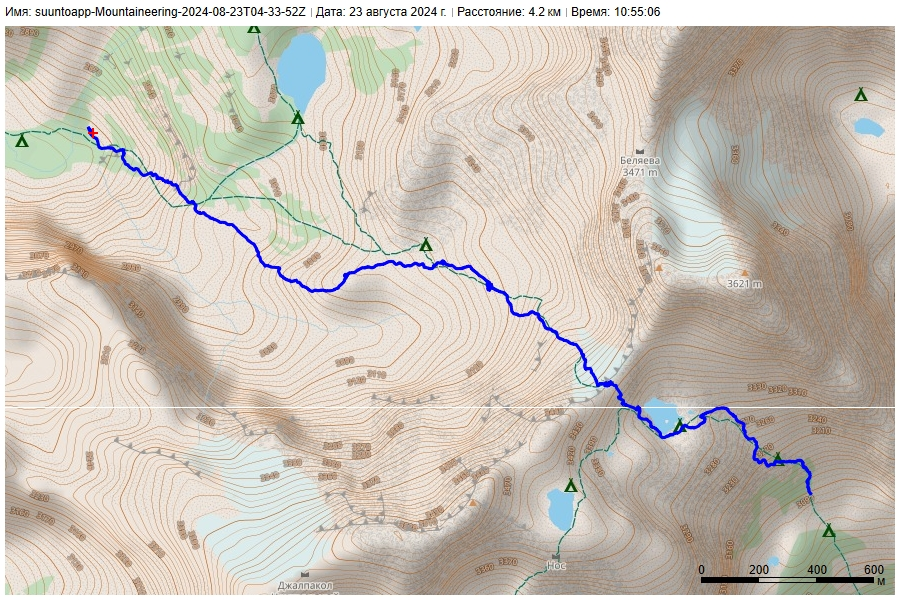
\includegraphics[angle=0, width=0.7\linewidth]{../pics/mini_maps/23}
	\label{fig:mini_23}
\end{figure}


Подъём в 04:30, выход в 07:30. С места ночёвки идёт подъем на моренный вал по помеченной турами тропе (рис.~\ref{fig:23augstart}). В 08:50 оказываемся на развилке троп (левая пхд тропа ведёт на каскадные озёра). Встречаем семейную пару туристов, которые спускались с перевала через эти озера. На развилке делаем привал, на котором Наташа заклеивает колено тейп-лентой и надевает наколенник.

\begin{figure}[h!]
	\centering
	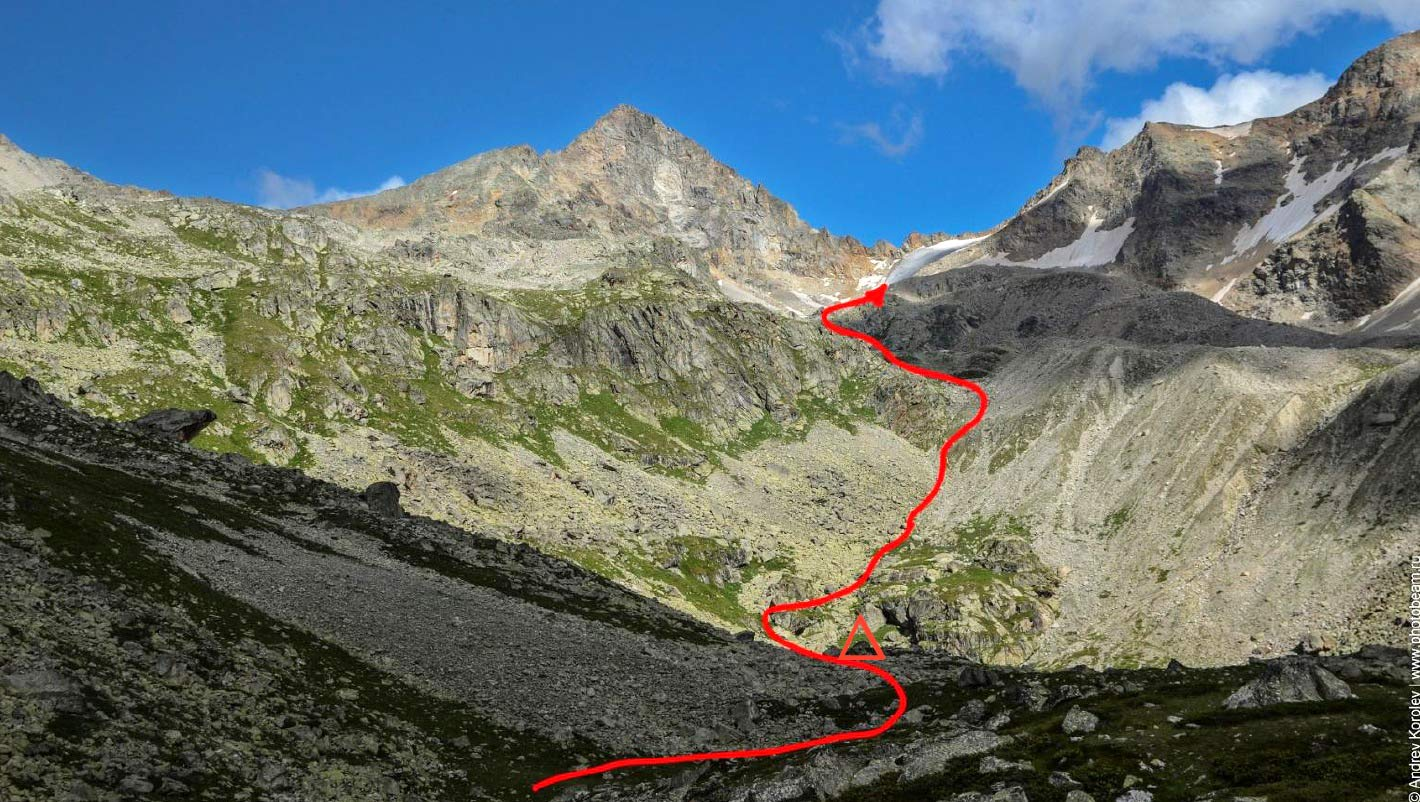
\includegraphics[angle=0, width=0.7\linewidth]{../pics/23augstart}
	\caption{Путь подъёма к перевалу Джалпаккол Северный от места ночёвки. Фото из отчёта Королёва А.Э. \cite{Korolyov2018}}
	\label{fig:23augstart}
\end{figure}

 Далее путь проходит по гребню моренного вала по слабомаркированной турами тропе. В 13:16 подходим под перевальный взлёт. Снега практически нет, ледник полностью открыт (рис.~\ref{fig:dzh_1}). Принимаем решение двигаться по правому пхд борту ледника. Как оказалось позднее, стандартный путь на этот перевал в виде <<крюка>> проходит ещё правее, но в нашем случае, когда снега на перевале не было, он проходил бы по осыпи, что только затруднило бы движение.
 



\begin{figure}[h!]
	\centering
	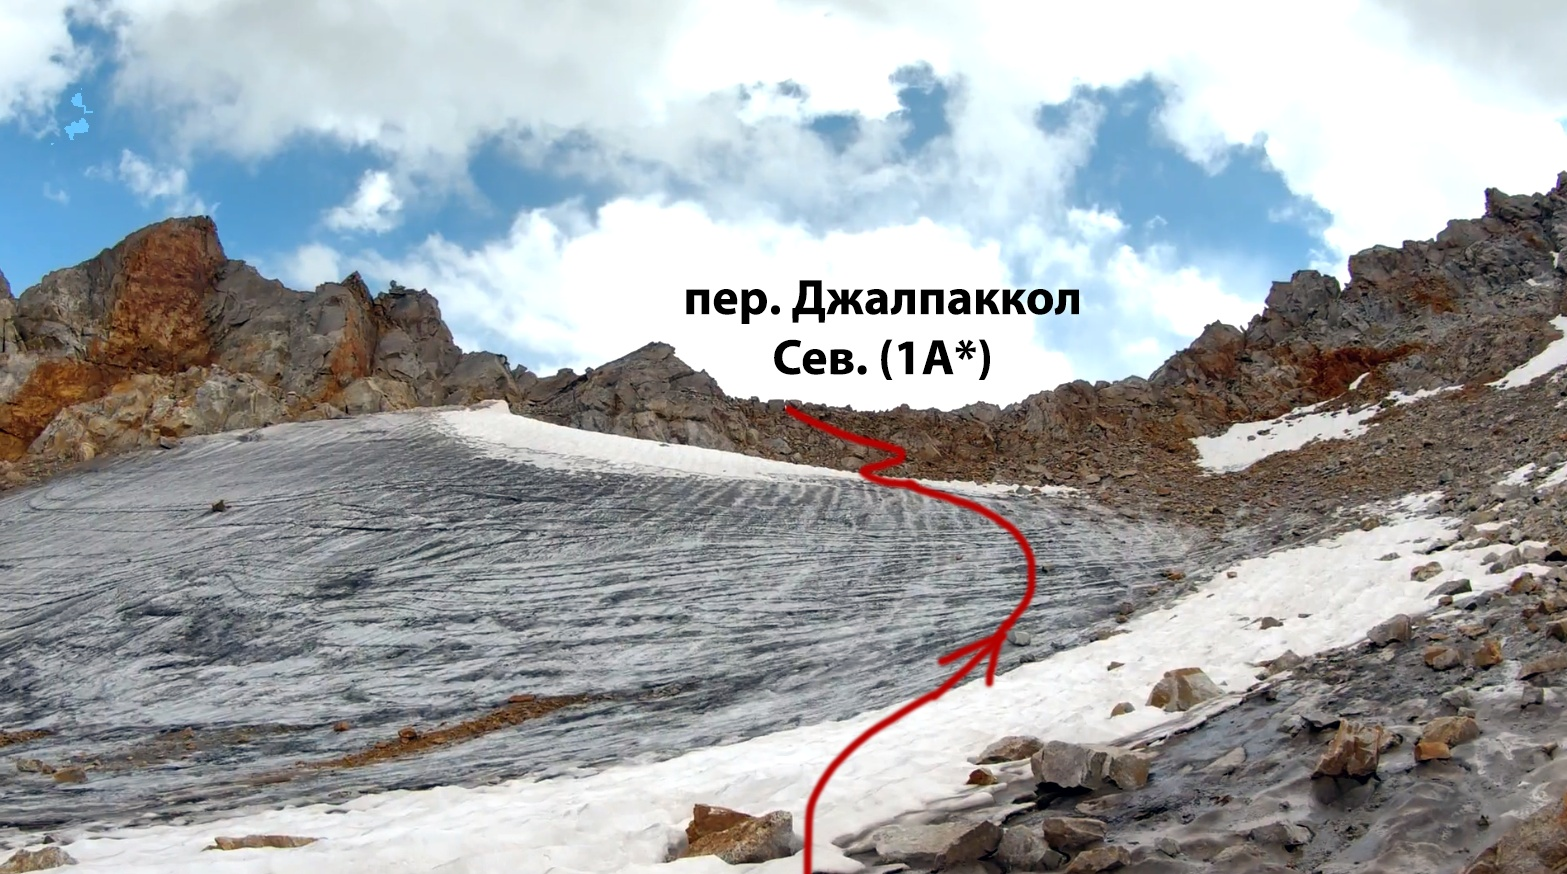
\includegraphics[width=0.7\linewidth]{../pics/dzh_1}
	\caption{Перевальный взлёт пер. Джалпаккол Северный}
	\label{fig:dzh_1}
\end{figure}

\begin{figure}[h!]	
	\centering
	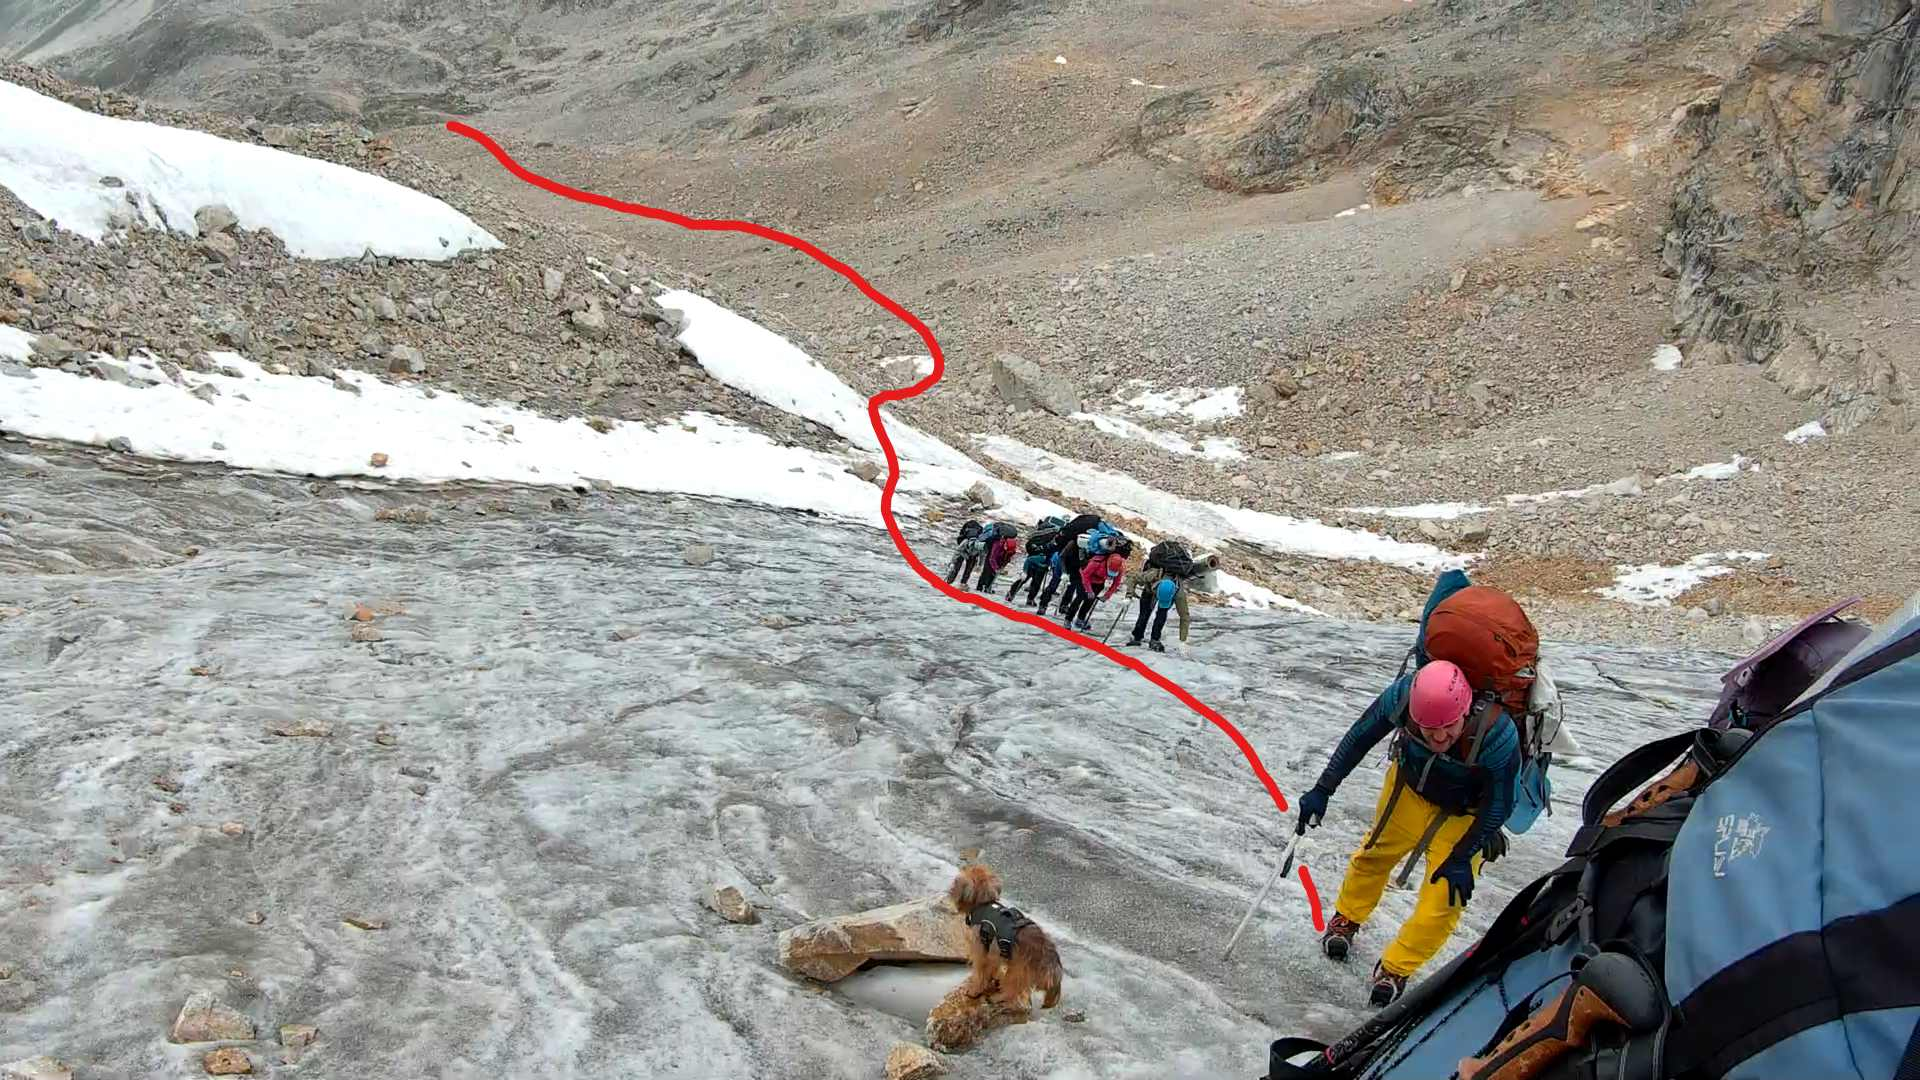
\includegraphics[angle=0, width=0.7\linewidth]{../pics/gopro_dzh}
	\caption{Подъём по леднику}
	\label{fig:gopro_dzh}
\end{figure}

\begin{figure}[h!]	
	\centering
	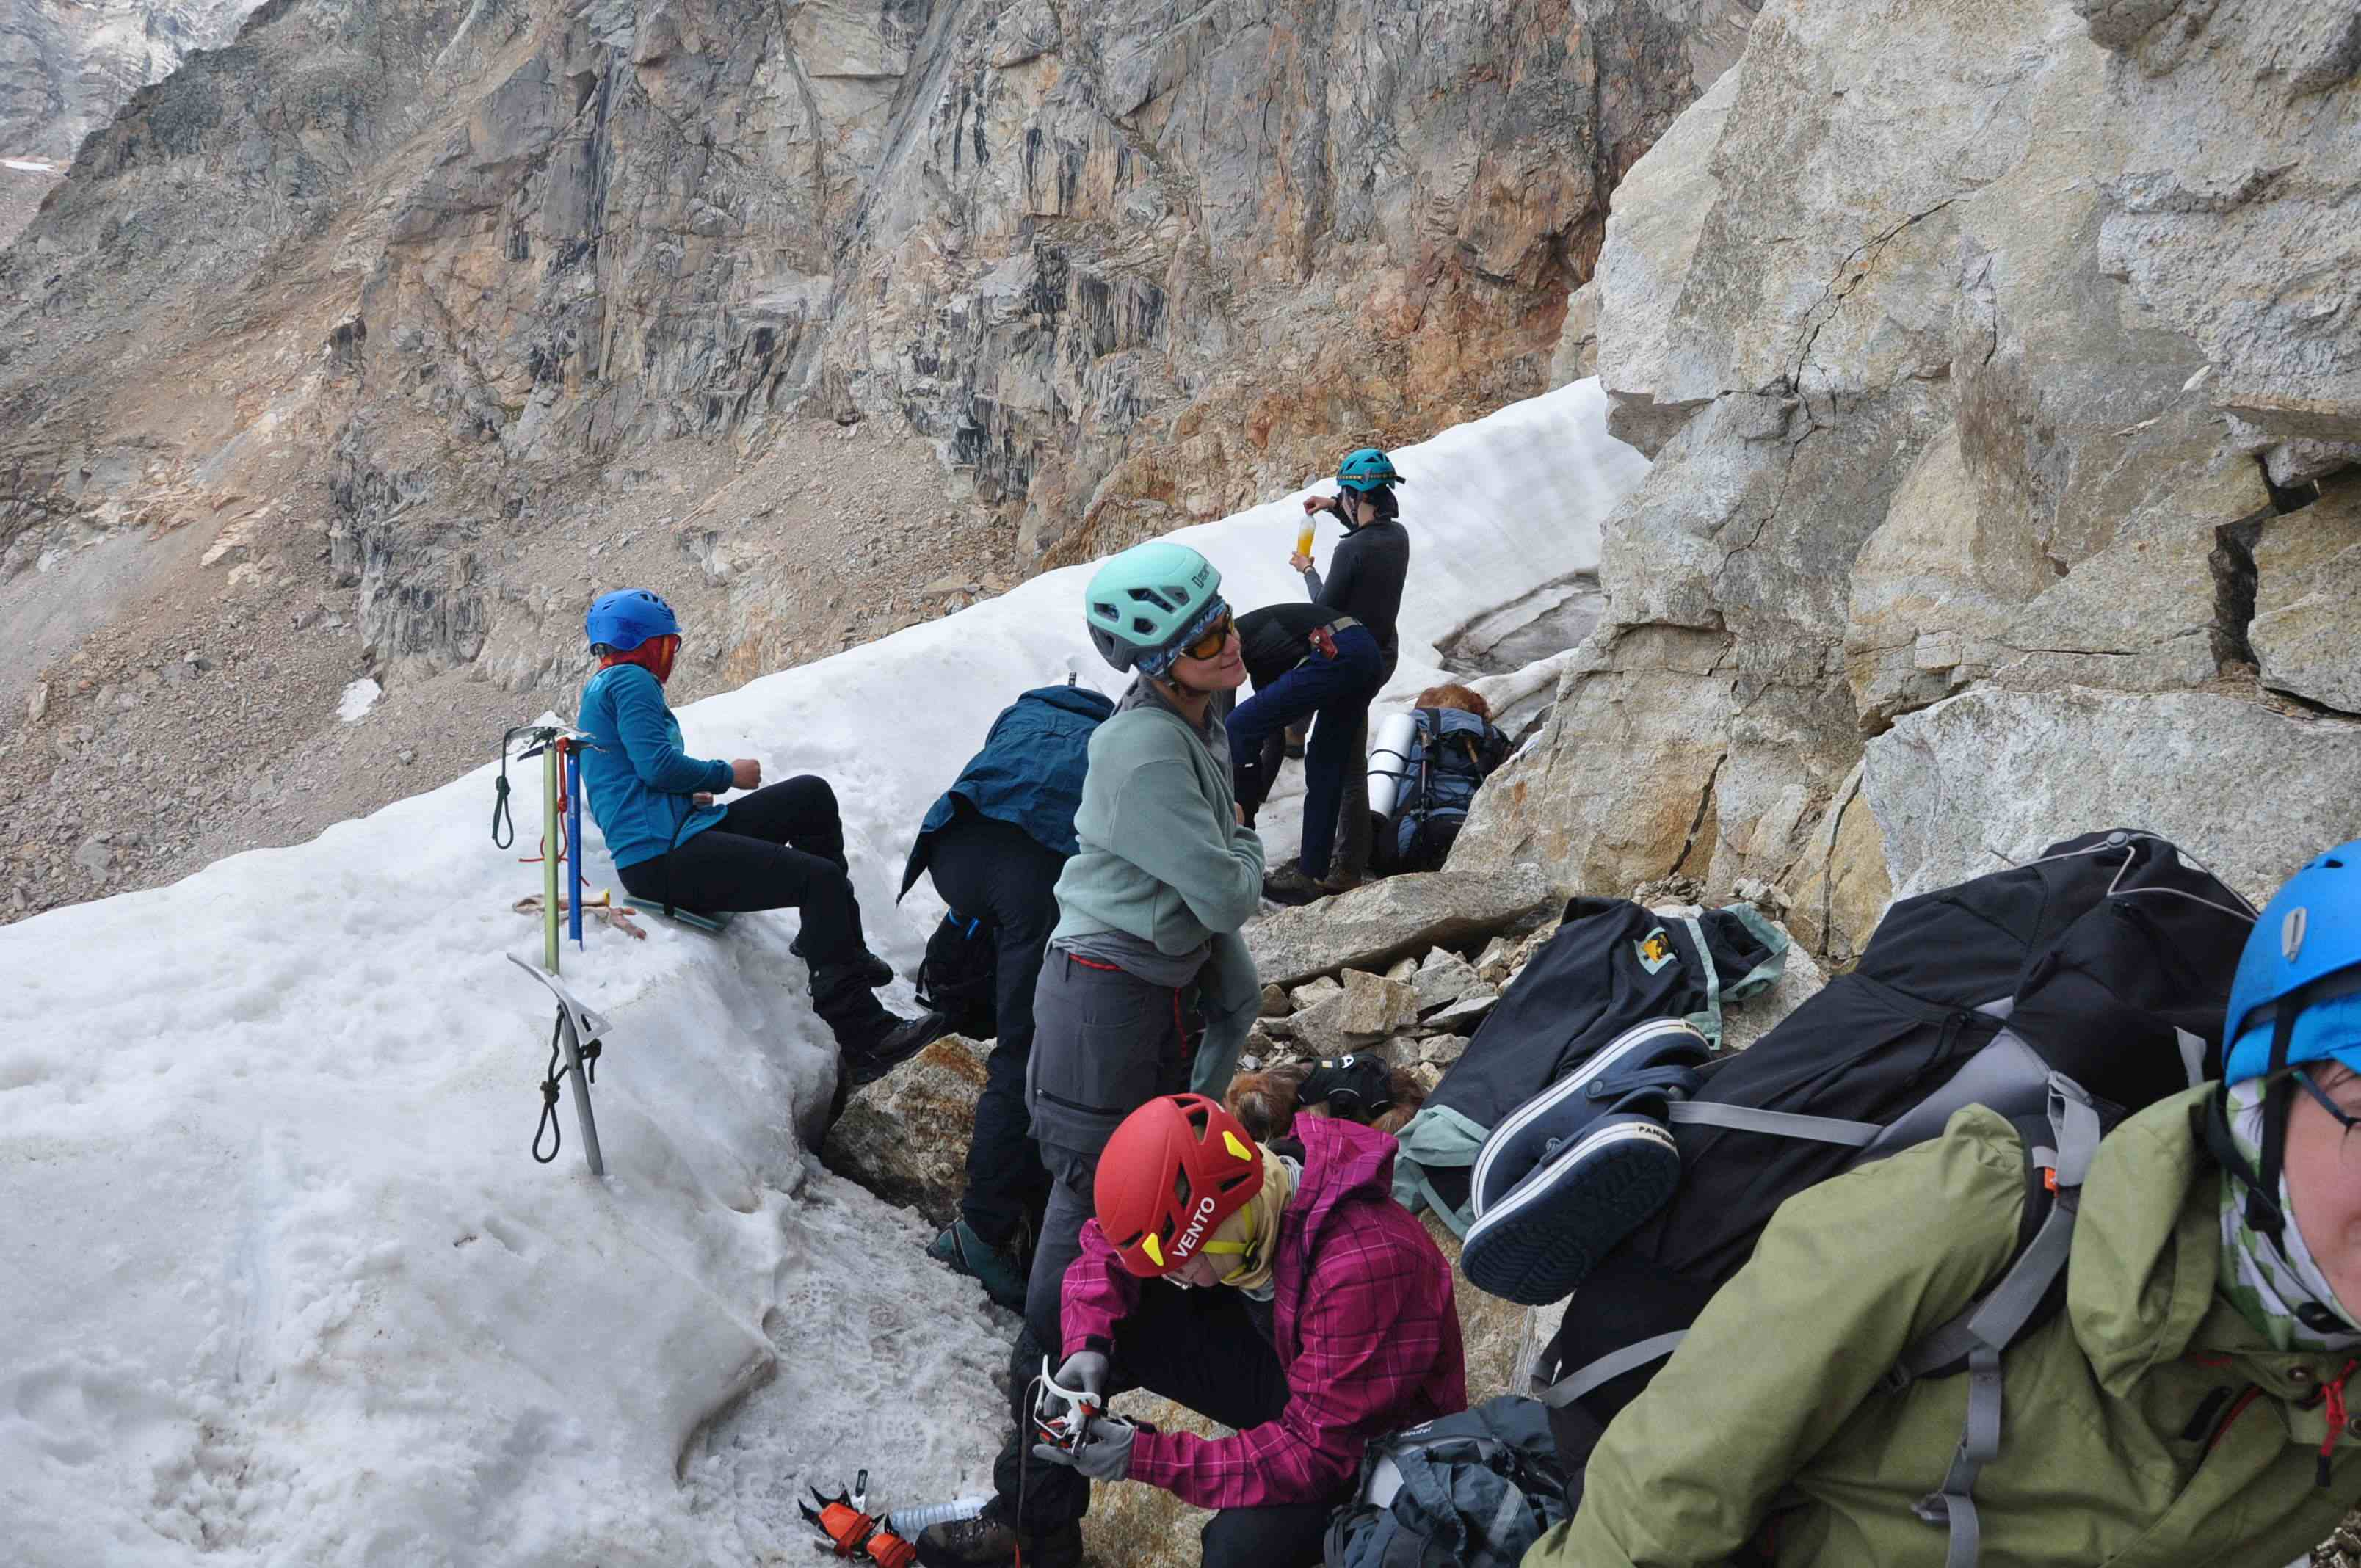
\includegraphics[angle=0, width=0.7\linewidth]{../pics/DSC_0021}
	\caption{Группа перед скальным участком перевала}
	\label{fig:DSC_0021}
\end{figure}


Подъём по леднику занимает 20 минут (рис.~\ref{fig:gopro_dzh}), в 14:45 приходим под финальный участок перевала~--- 10 метров лазания по сильно разрушенным скалам (рис.~\ref{fig:DSC_0021}) и снимаем кошки.




 Погода была хорошая, тепло и солнечно. Основная часть подъёма проходит по курумнику, группа останавливается на привалы каждые 15 минут, привалы длятся 10 минут. В 13:17 группа доходит до ледника и останавливается на технический привал, чтобы надеть кошки и забинтовать ногу Наташе (у нее болело колено). В 14:28 вся группа закончила прохождение ледника, устроили привал, чтобы снять кошки.        

Далее нужно было залезть на скальный гребень (высота где-то 10 м). Сначала руководители забрались без рюкзаков, чтобы определить наиболее удобный и безопасный маршрут, затем участники залезали парами. В 15:08 все взошли на перевал. С перевала открывался вид на озеро и долину реки Мырды.











\newpage